\documentclass[12pt,oneside,a4paper]{report}

% ============================================================
% Norme redazionali applicate in questo preambolo:
%  - font Times New Roman (approssimato con Times/Nimbus via
%    mathptmx: rende il documento compilabile ovunque, senza
%    dipendere dai font Microsoft installati nel sistema. Se si
%    preferisce Arial, commentare mathptmx e usare il blocco
%    "Alternativa Arial" subito sotto)
%  - corpo 12pt (le note a piè di pagina sono automaticamente a
%    10pt con la classe "report" a 12pt: \footnotesize = 10pt)
%  - margini 2,5 cm su tutti i lati (pacchetto geometry)
%  - interlinea 1,5 (pacchetto setspace, \onehalfspacing)
% ============================================================

\usepackage{mathptmx} % Times New Roman (approssimato)

% --- Alternativa Arial: scommentare queste due righe e commentare mathptmx sopra ---
% \usepackage{helvet}
% \renewcommand{\familydefault}{\sfdefault}

\usepackage[utf8]{inputenc}
\usepackage[T1]{fontenc}
\usepackage[italian,provide=*]{babel} % provide=*: questa installazione TeX Live ha solo i dati
    % linguistici generici dell'italiano, non il file .ldf dedicato -- vedi tesi/README.md

\usepackage[top=2.5cm,bottom=2.5cm,left=2.5cm,right=2.5cm]{geometry}
\usepackage{setspace}
\onehalfspacing

\usepackage{graphicx}
\usepackage{xcolor}
\usepackage{booktabs}
\usepackage{tikz}
\usetikzlibrary{arrows.meta, positioning, fit, backgrounds}
\usepackage{hyperref}
\hypersetup{
    colorlinks=true,
    linkcolor=black,
    citecolor=black,
    urlcolor=blue,
    pdftitle={Un assistente RAG locale per l'assistenza universitaria},
}

% --- Nota di redazione: comando per segnalare punti da scrivere/completare.
% Cercare "\notaredazionale" nei file sorgente per trovare tutti i placeholder. ---
\newcommand{\notaredazionale}[1]{%
    \par\noindent{\color{gray!70!black}\itshape [NOTA PER LA STESURA --- #1]}\par\medskip
}

\title{%
    Un assistente RAG locale per l'assistenza universitaria\\[0.3em]
    \large progettazione e valutazione
}
\author{Michele Nardini}
\date{\today}

\begin{document}

\maketitle

\tableofcontents

\chapter{Introduzione}
\label{cap:introduzione}

Il sito web e la documentazione di un ateneo raccolgono un'enorme quantità di informazioni --- regolamenti, tasse,
scadenze, piani di studio, materiali didattici --- ma lo fanno in modo estremamente dispersivo: argomenti correlati
tra loro finiscono su pagine diverse, i documenti sono distribuiti su sezioni distinte del sito senza un percorso di
consultazione unico, e le informazioni cambiano da un anno accademico all'altro senza che sia sempre immediato
capire dove si trovi la versione aggiornata. Uno studente che cerca una risposta puntuale (\emph{``quando scade la
prima rata?''}) o composita (\emph{``quali sono le diverse modalità di pagamento?''}) si trova spesso a dover
incrociare più fonti per ricostruire un quadro coerente, con un dispendio di tempo non indifferente e un margine
concreto di errore di interpretazione.

A questa dispersione si aggiunge una seconda difficoltà, che riguarda gli studenti che per ragioni diverse faticano a
seguire le lezioni con regolarità: per loro, un assistente capace di rispondere anche su contenuti didattici --- non
solo su procedure amministrative --- rappresenta un supporto concreto per recuperare e comprendere quanto trattato a
lezione, anche senza avervi potuto assistere di persona. Lo stesso tipo di supporto porta con sé un beneficio
speculare per i docenti: chi tiene più corsi, spesso con un numero elevato di studenti iscritti, fatica a propria
volta a rispondere individualmente a tutte le domande che riceve, molte delle quali ricorrenti e già risposte in
precedenza ad altri studenti. Un assistente che risponde autonomamente alle domande più comuni allegerisce questo
carico, lasciando ai docenti le domande che richiedono davvero la loro attenzione diretta.

La soluzione proposta in questo lavoro di tesi è un assistente conversazionale basato sul paradigma del
\emph{Retrieval-Augmented Generation} (RAG). A fronte di una domanda posta in linguaggio naturale, il sistema
recupera automaticamente, tra tutta la documentazione e il materiale didattico indicizzato, i frammenti più
pertinenti alla domanda posta, e li fornisce a un modello linguistico incaricato di formulare una risposta diretta
basandosi su di essi, citando la fonte da cui ogni affermazione proviene. In questo modo chi pone la domanda --- sia
esso uno studente o un docente che voglia verificare rapidamente un'informazione --- non deve più cercare manualmente
tra le pagine del sito o i materiali del corso: riceve una risposta puntuale e, soprattutto, verificabile, perché
ancorata a un documento reale e non semplicemente generata liberamente dal modello.

Il presente lavoro ha natura di \textbf{studio di fattibilità}: l'obiettivo primario non è consegnare un sistema
pronto per il deployment in produzione, ma verificare se un assistente di questo tipo --- completamente locale,
vincolato a un hardware non professionale --- possa rispondere con una qualità sufficiente a domande reali in questo
dominio, e individuare concretamente dove e perché un simile approccio fatica o fallisce. I contributi di questo
lavoro sono, di conseguenza: la progettazione e l'implementazione di un assistente RAG completamente locale per il
dominio universitario; un dataset diagnostico costruito appositamente per isolare le cause di errore lungo l'intera
pipeline, dal recupero alla generazione; un confronto sperimentale tra più modelli linguistici open-weight eseguibili
sull'hardware disponibile; l'identificazione e la risoluzione di una serie di problematiche concrete emerse durante
lo sviluppo, documentate insieme al processo diagnostico che le ha portate alla luce.

Il resto di questo lavoro di tesi è organizzato come segue. Il Capitolo~\ref{cap:stato-arte} inquadra il problema
nella letteratura esistente, introduce i concetti alla base dei modelli linguistici di grandi dimensioni e del
paradigma RAG, e passa in rassegna sistemi esistenti che affrontano problemi analoghi in ambito universitario. Il
Capitolo~\ref{cap:architettura} discute i vincoli di progetto che hanno guidato le scelte realizzative e descrive in
dettaglio l'architettura del sistema sviluppato, le scelte tecnologiche operate per ciascun componente e le
problematiche concrete incontrate durante lo sviluppo, insieme alle soluzioni adottate per risolverle. Il
Capitolo~\ref{cap:validazione} presenta la metodologia di valutazione sperimentale impiegata, gli esperimenti
condotti e i risultati ottenuti, inclusi alcuni casi di errore analizzati in dettaglio. Il
Capitolo~\ref{cap:conclusioni}, infine, riassume il contributo di questo lavoro rispetto agli obiettivi qui
enunciati, ne discute i limiti noti e ne delinea i possibili sviluppi futuri.

\chapter{Stato dell'arte}
\label{cap:stato-arte}

\notaredazionale{Obiettivo: 15 pagine complessive per l'intero capitolo.}

\section{Il problema da affrontare}
\label{sec:problema}

Un modello linguistico di grandi dimensioni, per quanto addestrato su un corpus sterminato di testo, soffre di due
limiti strutturali quando interrogato direttamente su un dominio specifico e circoscritto come quello universitario.

Il primo è la natura statica della sua conoscenza: i parametri del modello fissano ciò che esso ``sa'' al momento in
cui l'addestramento si conclude, e qualunque informazione successiva a quella data --- una nuova scadenza, un
regolamento modificato, un importo delle tasse aggiornato --- semplicemente non vi rientra. Zhao et al.
\cite{zhao2023survey}, nella loro rassegna sui large language model, descrivono questo fenomeno con il termine
\emph{outdatedness hallucination}: il modello genera un contenuto che era corretto al momento dell'addestramento ma
non lo è più al momento dell'uso, senza alcun segnale esplicito che lo distingua da un'affermazione ancora valida ---
il modello stesso non ha modo di sapere che la propria conoscenza è invecchiata.

Il secondo limite riguarda l'assenza totale di accesso ai documenti specifici dell'istituzione interrogata: un LLM
generico non ha mai visto i regolamenti di un ateneo, le pagine web di un singolo corso di laurea, le slide di un
insegnamento particolare. Messo di fronte a una domanda che richiede questo tipo di conoscenza, non ha altra scelta
che generalizzare da pattern appresi su domini affini o, più problematicamente, produrre una risposta sintatticamente
corretta e sicura di sé ma priva di fondamento fattuale --- un comportamento ampiamente documentato in letteratura
sotto il nome di \emph{hallucination}. Huang et al. \cite{huang2023survey} ne propongono una tassonomia sistematica,
riconducendone le cause a limiti dei dati di addestramento (rumorosi, incompleti o distorti), a processi di
allineamento che premiano risposte sicure più che corrette, e alla natura intrinsecamente stocastica del processo di
generazione del testo.

Questa tassonomia, per quanto utile a inquadrare il fenomeno in astratto, non distingue ancora i modi concreti in cui
un sistema di questo tipo può fallire su un dominio specifico --- una distinzione che si rivela necessaria nel
momento in cui occorre costruire un dataset di valutazione, piuttosto che limitarsi a discutere il problema in linea
di principio. Il dataset diagnostico impiegato in questo lavoro (Capitolo~\ref{cap:validazione}) riflette proprio
questa necessità, isolando categorie di domande distinte per il tipo di fallimento che sono pensate a far emergere:
domande la cui risposta corretta dipende dal riconoscere una negazione implicita nella richiesta
(\texttt{qualitative\_negation}), domande che richiedono di sintetizzare informazione sparsa su più frammenti
(\texttt{synthesis}), domande a cui il sistema dovrebbe correttamente astenersi dal rispondere perché fuori dal
dominio indicizzato (\texttt{out\_of\_scope}) o perché l'informazione richiesta non è presente nei documenti
(\texttt{no\_information}), e domande la cui risposta richiede di interpretare un'immagine piuttosto che solo testo
(\texttt{image\_grounded}) --- quest'ultima categoria discussa anche nella Sottosezione~\ref{subsec:llm-valutati} a
proposito della scelta dei modelli generativi. Un errore in una qualunque di queste categorie può manifestarsi
superficialmente come la stessa ``risposta plausibile ma sbagliata'' descritta da Huang et al., ma avere un'origine
diagnosticamente distinta --- una distinzione che la sola tassonomia della letteratura non rende, e che motiva la
scelta di costruire un dataset ad hoc piuttosto che affidarsi a un benchmark generico di hallucination detection.

Questi due limiti si combinano in modo particolarmente dannoso nel dominio universitario, dove il costo di un errore
non è astratto ma concreto e misurabile: una scadenza riportata in modo errato comporta una tassa pagata in ritardo,
un requisito di ammissione frainteso comporta una domanda respinta. Kasneci et al. \cite{kasneci2023chatgpt},
discutendo opportunità e criticità dell'uso dei large language model in ambito educativo, osservano come l'assenza di
garanzie sull'accuratezza fattuale sia uno degli ostacoli principali alla loro adozione diretta in contesti dove la
correttezza dell'informazione fornita allo studente non è negoziabile.

La soluzione che la letteratura ha individuato per entrambi questi limiti consiste nel separare la conoscenza
fattuale dal componente che genera il linguaggio: non chiedere al modello di ``ricordare'' un fatto a partire dai
propri parametri, ma fornirglielo esplicitamente come contesto al momento della domanda, recuperandolo da una base
documentale aggiornabile in modo indipendente dal modello stesso. È il principio alla base del
Retrieval-Augmented Generation, discusso nella Sezione~\ref{sec:rag}, ed è il principio su cui si fonda l'intero
sistema sviluppato in questo lavoro di tesi (si veda anche \texttt{REPORT\_ARCHITETTURA.md} \S1.3--1.4).

Questa non è l'unica strada percorribile: la conoscenza mancante di un LLM potrebbe, in linea di principio, essere
aggiunta direttamente ai suoi parametri con un ulteriore addestramento mirato (\emph{fine-tuning}) sui documenti
specifici del dominio, piuttosto che recuperata da una base esterna a ogni domanda. Ovadia et al.
\cite{ovadia2024finetuning} confrontano empiricamente le due strade su compiti che richiedono conoscenza intensiva,
sia per informazioni già presenti nei dati di addestramento sia per informazioni del tutto nuove, e osservano che il
fine-tuning non supervisionato fatica sistematicamente ad apprendere fatti nuovi in modo affidabile --- a meno di
esporre il modello a numerose riformulazioni dello stesso fatto durante l'addestramento, un costo che cresce con
ogni aggiornamento del documento sorgente --- mentre il RAG si dimostra costantemente più efficace in entrambi i
casi. Per un dominio come quello universitario, dove i documenti cambiano ogni anno accademico, questo risultato ha
un peso pratico diretto: un sistema a fine-tuning richiederebbe un nuovo ciclo di addestramento a ogni aggiornamento
normativo, mentre un sistema RAG richiede solo di re-indicizzare il documento modificato.

Questo principio ha già trovato applicazione in sistemi conversazionali rivolti specificamente al contesto
universitario. Marcel, sviluppato per supportare gli studenti dell'Università di Marburg, affronta un problema
affine --- rispondere a domande di studenti prospettivi sulle procedure di ammissione --- integrando nella pipeline
di recupero un componente dedicato alle domande frequenti, che consente al personale amministrativo di orientare
esplicitamente cosa il sistema recupera per le domande più comuni \cite{trienes2025marcel}. Una rassegna più ampia di
sistemi analoghi, inclusi i confronti con soluzioni commerciali che si affidano all'autenticazione istituzionale per
disambiguare il profilo dello studente, è presentata nella Sezione~\ref{sec:sistemi-simili}.

\section{Large Language Model (LLM)}

\subsection{Descrizione sintetica di cosa è un LLM}
\label{subsec:llm-desc}

Un \emph{large language model} è, nella sua forma più diffusa, una rete neurale basata sull'architettura
\emph{Transformer} \cite{vaswani2017attention}, addestrata a predire il token successivo di una sequenza di testo a
partire da un contesto precedente. L'elemento che ha reso questa architettura dominante rispetto ai modelli
ricorrenti che la precedevano è il meccanismo di \emph{self-attention}: ogni token della sequenza viene messo in
relazione diretta con tutti gli altri, indipendentemente dalla loro distanza, permettendo al modello di catturare
dipendenze a lungo raggio nel testo senza il collo di bottiglia sequenziale delle reti ricorrenti e, soprattutto,
abilitando un addestramento parallelizzabile su hardware specializzato --- una condizione necessaria per scalare
questi modelli alle dimensioni, in termini di parametri e di dati di addestramento, che li caratterizzano oggi.

L'addestramento di un LLM avviene tipicamente in due fasi distinte. Nella fase di \emph{pre-training}, il modello
viene esposto a un corpus testuale di dimensioni enormi --- miliardi o migliaia di miliardi di token raccolti dal web,
da libri, da codice sorgente --- con il solo obiettivo di predire il token successivo; da questa fase, puramente
auto-supervisionata e priva di etichette fornite da un umano, emerge la competenza linguistica e una parte
significativa della conoscenza fattuale del modello, codificata implicitamente nei suoi parametri \cite{zhao2023survey}.
Un modello che ha completato solo questa fase, tuttavia, non è ancora un assistente conversazionale: è un sistema di
completamento testuale, che tende a proseguire il prompt ricevuto piuttosto che a rispondere a una domanda o a
eseguire un'istruzione. La seconda fase, l'\emph{instruction-tuning}, affina il modello pre-addestrato su coppie
istruzione-risposta e, spesso, su un segnale di preferenza umana raccolto successivamente (\emph{reinforcement
learning from human feedback}, RLHF): Ouyang et al. \cite{ouyang2022instructgpt}, nel lavoro che ha introdotto
InstructGPT, mostrano come questa seconda fase sia determinante tanto quanto la scala del modello stesso nel renderlo
utile e sicuro da un punto di vista comportamentale --- un modello InstructGPT da 1,3 miliardi di parametri viene
preferito da valutatori umani a un modello GPT-3 da 175 miliardi di parametri non sottoposto a questo affinamento. È
questa seconda fase che rende un LLM capace di rispondere in modo pertinente, nella forma, a una domanda posta in
linguaggio naturale; resta però, come discusso nella Sezione~\ref{sec:problema}, incapace di garantire che il
contenuto della risposta sia corretto o aggiornato, un limite che l'instruction-tuning non affronta perché riguarda
la conoscenza codificata nei parametri, non il comportamento del modello.

\begin{figure}[htbp]
  \centering
  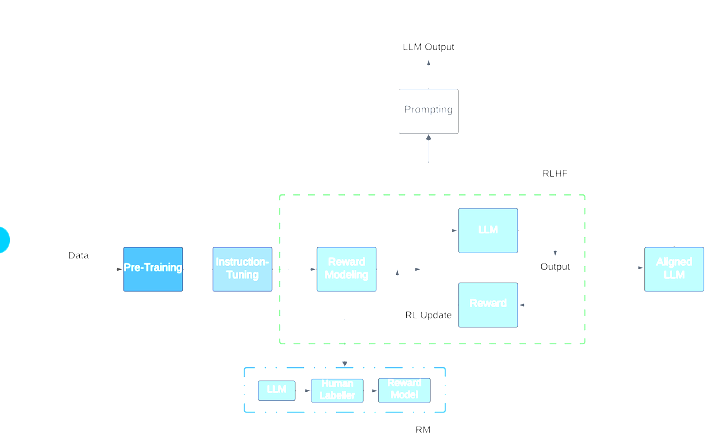
\includegraphics[width=0.85\textwidth]{capitoli/immagini/llm-training-pipeline.png}
  \caption{Le fasi che portano dai dati grezzi a un LLM allineato e utilizzabile tramite prompting: pre-training,
    instruction-tuning e, infine, l'allineamento tramite \emph{reward modeling} (RM, in basso: un modello di
    ricompensa addestrato su confronti prodotti da annotatori umani) e \emph{reinforcement learning from human
    feedback} (RLHF, al centro: un ciclo iterativo che aggiorna l'LLM in base al segnale del modello di ricompensa).
    Adattata da Naveed et al. \cite{naveed2023overview}, Figura 6.}
  \label{fig:llm-training}
\end{figure}

La Figura~\ref{fig:llm-training} riassume questo percorso in tre fasi anziché due: oltre al pre-training e
all'instruction-tuning già discussi, mostra esplicitamente anche la fase di \emph{allineamento} tramite RLHF ---
il meccanismo con cui Ouyang et al. \cite{ouyang2022instructgpt} affinano il modello sulla base di un segnale di
preferenza umana, qui scomposto nei suoi due componenti (l'addestramento del modello di ricompensa a partire da
confronti annotati da umani, e il ciclo di aggiornamento del modello linguistico guidato da quella ricompensa). È
importante notare che la conoscenza fattuale del modello si forma quasi interamente nella prima fase (pre-training),
mentre le fasi successive ne modificano il comportamento senza aggiungere --- se non marginalmente --- nuova
conoscenza.

Due aspetti più tecnici, rilevanti per le scelte discusse nella sezione successiva, meritano una menzione. Il primo è
la tokenizzazione: un LLM non elabora direttamente caratteri o parole, ma \emph{token}, unità sub-lessicali ottenute
segmentando il testo con un algoritmo di compressione appreso sul corpus di addestramento; la \emph{finestra di
contesto} del modello --- il numero massimo di token che può elaborare in un'unica interazione, da poche migliaia a
centinaia di migliaia a seconda del modello --- pone un limite diretto a quanto testo recuperato (Sezione~\ref{sec:rag})
può essere fornito come contesto per una singola domanda. Il secondo è la relazione, osservata empiricamente da
Kaplan et al. \cite{kaplan2020scaling} ancor prima della diffusione dei moderni LLM conversazionali, tra la
dimensione di un modello (numero di parametri), la quantità di dati di addestramento e la potenza di calcolo
impiegata nell'addestramento da un lato, e la qualità delle sue previsioni dall'altro: un andamento a legge di
potenza, via via più favorevole al crescere di tutti e tre i fattori insieme. È questa relazione --- oggi nota come
\emph{scaling law} --- a motivare l'esistenza stessa di famiglie di modelli a più taglie, come Qwen2.5-14B e
Qwen2.5-7B discussi nella sezione seguente: a parità di architettura e dati di addestramento, un modello più grande è
sistematicamente più capace, al costo di maggiore memoria e tempo di calcolo per ogni risposta generata --- il
compromesso al centro del confronto sperimentale di questo lavoro (Capitolo~\ref{cap:validazione}).

Un'ultima capacità, distinta sia dal pre-training sia dall'instruction-tuning, è rilevante per inquadrare il
funzionamento di un sistema RAG come quello di questo lavoro: l'\emph{in-context learning}. Brown et al.
\cite{brown2020gpt3}, presentando GPT-3, osservano che un modello linguistico sufficientemente grande può adattare
il proprio comportamento a un compito nuovo semplicemente a partire da istruzioni o esempi forniti nel testo del
prompt stesso, senza alcun aggiornamento dei suoi parametri --- una capacità che emerge dalla sola scala del modello,
osservabile già nel modello pre-addestrato prima di qualunque instruction-tuning. È precisamente questo meccanismo,
e non un nuovo addestramento, che un sistema RAG sfrutta quando fornisce al modello un contesto recuperato al momento
della domanda (Sezione~\ref{sec:rag}): il modello non apprende un fatto nuovo in modo permanente, ma lo usa
temporaneamente, limitatamente alla singola interazione in cui compare nel prompt.

Ai fini di questo lavoro è rilevante anche la distinzione tra modelli \emph{closed-weight}, accessibili solo tramite
un'interfaccia remota a pagamento gestita dal fornitore, e modelli \emph{open-weight}, i cui parametri sono
pubblicati e possono essere eseguiti su hardware proprio. Il vincolo di riservatezza del progetto (§1.2 di
\texttt{REPORT\_ARCHITETTURA.md}) esclude a priori la prima categoria: tutti i modelli generativi considerati in
questo lavoro, descritti nella sezione seguente, sono modelli open-weight eseguibili interamente in locale.

\subsection{LLM valutati}
\label{subsec:llm-valutati}

Il sistema sviluppato in questo lavoro è stato valutato con quattro modelli generativi open-weight, scelti per essere
eseguibili sull'hardware a disposizione (§3.1 di \texttt{REPORT\_ARCHITETTURA.md}) a condizione di ricorrere a una
quantizzazione a precisione ridotta. Tutti e quattro sono serviti nella variante \emph{AWQ} (\emph{Activation-aware
Weight Quantization}), uno schema di quantizzazione post-addestramento a 4 bit che Lin et al. \cite{lin2024awq}
propongono osservando che una piccola frazione dei pesi di un modello --- quelli associati ai canali di attivazione
di ampiezza maggiore --- contribuisce in modo sproporzionato all'errore di quantizzazione: proteggendo selettivamente
questi pesi salienti, individuati dalle statistiche di attivazione piuttosto che dalla sola magnitudine dei pesi, è
possibile ridurre drasticamente la perdita di qualità rispetto a uno schema di quantizzazione uniforme, senza
richiedere un nuovo addestramento né una fase di backpropagation.

\begin{table}[htbp]
  \centering
  \small
  \begin{tabular}{@{}lccccc@{}}
    \toprule
    \textbf{Modello} & \textbf{Parametri} & \textbf{Contesto} & \textbf{Token pre-training} & \textbf{Multimodale} & \textbf{Sviluppatore} \\
    \midrule
    Qwen2.5-14B-Instruct      & 14 mld & 128k & 18.000 mld & Sì & Alibaba Cloud \\
    Qwen2.5-7B-Instruct       & 7 mld  & 128k & 18.000 mld & Sì & Alibaba Cloud \\
    Mistral-Nemo-Instruct-12B & 12 mld & 128k & n.d.\footnotemark & No & Mistral AI / NVIDIA \\
    Meta-Llama-3.1-8B-Instruct & 8 mld & 128k & $>$15.000 mld & No & Meta \\
    \bottomrule
  \end{tabular}
  \caption{Confronto dei quattro modelli generativi valutati in questo lavoro, secondo i rispettivi technical
    report/documentazione ufficiale \cite{qwen2024technical, mistralai2024nemo, grattafiori2024llama3}. Tutti e
    quattro sono serviti in questo progetto nella variante quantizzata AWQ a 4 bit \cite{lin2024awq}; la capacità
    multimodale si riferisce alla versione non quantizzata del modello.}
  \label{tab:llm-confronto}
\end{table}
\footnotetext{Il numero esatto di token di pre-training non è dichiarato nella documentazione pubblica di Mistral NeMo.}

La Tabella~\ref{tab:llm-confronto} riassume i parametri quantitativi dei quattro modelli; i paragrafi seguenti ne
descrivono le caratteristiche qualitative più rilevanti per questo lavoro. I quattro modelli confrontati sono:

\begin{itemize}
  \item \textbf{Qwen2.5-14B-Instruct-AWQ} e \textbf{Qwen2.5-7B-Instruct-AWQ}, due varianti per dimensione della
    famiglia Qwen2.5 sviluppata da Alibaba Cloud \cite{qwen2024technical}. Gli autori riportano un corpus di
    pre-training di 18 mila miliardi di token --- più del doppio dei 7 mila miliardi della generazione precedente
    (Qwen2) --- con un'attenzione dichiarata particolare a codice e matematica, oltre a un supporto multilingue esteso
    a decine di lingue secondo la documentazione del fornitore. Entrambe le varianti dichiarano una finestra di
    contesto di 128k token e sono multimodali (capaci di comprensione visiva oltre che testuale) nella loro versione
    non quantizzata, pur differendo di un fattore 2 nel numero di parametri (14 contro 7 miliardi) --- la coppia
    pensata in questo lavoro per isolare l'effetto della sola dimensione a parità di famiglia e dati di addestramento;
  \item \textbf{Mistral-Nemo-Instruct-12B-AWQ}, sviluppato congiuntamente da Mistral AI e NVIDIA
    \cite{mistralai2024nemo}, un modello da 12 miliardi di parametri con finestra di contesto estesa (128k token) ma
    privo di capacità multimodali. Introduce un nuovo tokenizzatore (Tekken), che gli autori riportano essere più
    efficiente di circa il 30\% rispetto ai tokenizzatori usati dai modelli concorrenti su codice sorgente e sulla
    maggior parte delle lingue supportate (fino al doppio o al triplo per coreano e arabo), ed è stato addestrato con
    \emph{quantization awareness}, una procedura pensata per permettere un'inferenza a precisione ridotta (FP8) senza
    perdita di qualità percepibile --- un obiettivo di design affine, pur se non identico nella tecnica, a quello che
    motiva l'uso di AWQ in questo lavoro;
  \item \textbf{Meta-Llama-3.1-8B-Instruct}, appartenente alla famiglia Llama 3 di Meta \cite{grattafiori2024llama3},
    anch'esso privo di comprensione visiva nella variante considerata. Fa parte di una famiglia di tre taglie dense
    (8, 70 e 405 miliardi di parametri, nessuna delle quali a mixture-of-experts), addestrate su oltre 15 mila
    miliardi di token con una finestra di contesto nativa di 128k token; gli autori dichiarano un supporto ufficiale
    esplicito per otto lingue e un addestramento specifico per l'uso di strumenti esterni (\emph{tool calling}), una
    capacità agentica non direttamente rilevante per l'uso che ne fa questo sistema, puramente conversazionale.
\end{itemize}

Tutti e quattro condividono la stessa architettura di fondo (Transformer decoder-only autoregressivo, descritta nella
Sottosezione~\ref{subsec:llm-desc}) e differiscono principalmente per numero di parametri, dati e procedura di
addestramento, e finestra di contesto: Qwen2.5-14B/7B e Llama-3.1-8B
dichiarano una finestra di 128k token, pari a quella di Mistral-Nemo-12B già citata; nessuno dei quattro adotta
un'architettura a \emph{mixture-of-experts} (con solo una parte dei parametri attiva per ogni token, una tecnica
impiegata da altri modelli della stessa epoca per aumentare la capacità senza aumentare proporzionalmente il costo di
inferenza) --- una scelta che semplifica il confronto sperimentale del Capitolo~\ref{cap:validazione}, perché isola
l'effetto della dimensione e della famiglia del modello senza introdurre una variabile architetturale aggiuntiva.

La scelta di includere sia modelli con sia senza capacità di comprensione visiva non è incidentale: una parte dei
documenti indicizzati dal sistema (slide, schemi, diagrammi) ha contenuto prevalentemente visivo, e la Sezione~6.3 del
Capitolo~\ref{cap:validazione} mostra come questa capacità incida in modo misurabile sulla qualità delle risposte a
domande che richiedono di interpretare un'immagine. Il confronto sistematico tra questi quattro modelli --- in
termini di qualità della risposta generata, latenza e comportamento sulle diverse categorie del dataset diagnostico
--- è presentato nel Capitolo~\ref{cap:validazione} (già raccolto in \texttt{REPORT\_ARCHITETTURA.md} \S6.3--6.4 e nei
file \texttt{datasets/eval/model\_comparison/*.json}); qui interessa solo caratterizzare i modelli come artefatti
della letteratura, non ancora i risultati del loro impiego in questo sistema.

\subsection{Servire un LLM in locale: l'inferenza}
\label{sec:inferenza}

Oltre alla qualità delle risposte, un vincolo pratico distinto pesa su un sistema che deve servire un LLM in locale,
su hardware proprio, a più utenti potenzialmente concorrenti: l'efficienza dell'inferenza. La generazione di un LLM è
intrinsecamente sequenziale --- ogni nuovo token dipende da tutti quelli generati in precedenza --- e per evitare di
ricalcolare da zero l'intera sequenza a ogni passo, i motori di inferenza mantengono in memoria una cache delle
rappresentazioni intermedie già calcolate dal meccanismo di attenzione (la \emph{KV cache}). Questa cache cresce con
la lunghezza della sequenza generata e, soprattutto, con il numero di richieste gestite in parallelo: una gestione
ingenua di questa memoria, allocata in blocchi contigui di dimensione fissa come avveniva nei motori di inferenza
precedenti, spreca una quota significativa della memoria disponibile per frammentazione interna, limitando
artificialmente quante richieste concorrenti un singolo modello può servire sulla stessa GPU.

Kwon et al. \cite{kwon2023vllm} affrontano questo problema con \emph{PagedAttention}, un algoritmo di attenzione che
gestisce la KV cache in blocchi non contigui, sul modello della paginazione della memoria virtuale nei sistemi
operativi, ed è alla base di vLLM, il motore di inferenza impiegato in questo progetto per servire tutti e quattro i
modelli generativi confrontati (\texttt{docker-compose.yml}; \texttt{REPORT\_ARCHITETTURA.md} \S3.1). Riducendo lo
spreco di memoria e abilitando un \emph{continuous batching} delle richieste --- l'inserimento di nuove richieste nel
batch di generazione senza attendere che quelle in corso terminino --- gli autori riportano un throughput 2--4 volte
superiore, a parità di latenza, rispetto ai motori di inferenza precedenti. Questo guadagno di efficienza non è un
dettaglio implementativo marginale rispetto al resto di questo lavoro: è precisamente ciò che rende praticabile,
sull'hardware a disposizione, l'obiettivo enunciato nell'Introduzione di alleggerire il carico di un docente che
riceve domande ricorrenti da un numero elevato di studenti, piuttosto che da un singolo utente alla volta.

\section{Retrieval-Augmented Generation (RAG)}
\label{sec:rag}

Il \emph{Retrieval-Augmented Generation} è il paradigma che Lewis et al. \cite{lewis2020retrieval} propongono per
superare i due limiti discussi nella Sezione~\ref{sec:problema}: invece di affidarsi esclusivamente alla conoscenza
codificata nei parametri del modello, il sistema recupera prima, da una base documentale esterna e aggiornabile
indipendentemente, i frammenti di testo più pertinenti alla domanda ricevuta, e li fornisce al modello linguistico
come contesto su cui basare la risposta. Il principio di fondo è separare nettamente \emph{cosa il sistema sa} ---
l'insieme dei documenti indicizzati, che può essere aggiornato in qualunque momento senza bisogno di un nuovo
addestramento --- da \emph{come il sistema si esprime}, compito che resta demandato interamente al modello
linguistico. Gao et al. \cite{gao2023ragsurvey}, nella loro rassegna sul tema, inquadrano questo principio come la
risposta più diretta proprio ai limiti di conoscenza statica e di verificabilità discussi in precedenza: un'affermazione
generata dal modello può essere ricondotta a un frammento di testo specifico, citabile e verificabile, invece che
derivare implicitamente e in modo opaco dai suoi parametri.

\begin{figure}[htbp]
  \centering
  \resizebox{\textwidth}{!}{%
  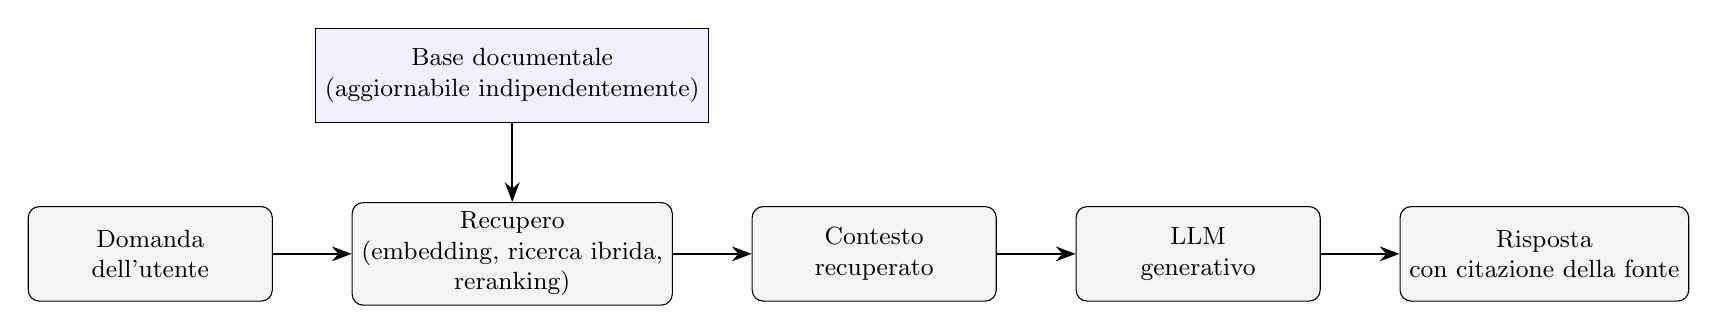
\begin{tikzpicture}[
      node distance=8mm and 10mm,
      box/.style={rectangle, draw, rounded corners, align=center, minimum height=1.2cm, minimum width=3.1cm,
                  fill=gray!8, font=\small},
      store/.style={rectangle, draw, align=center, minimum height=1.2cm, minimum width=3.1cm,
                    fill=blue!6, font=\small},
      arr/.style={-{Stealth[length=2.5mm]}, thick}
    ]
    \node[box] (query) {Domanda\\dell'utente};
    \node[box, right=of query] (retrieval) {Recupero\\(embedding, ricerca ibrida,\\reranking)};
    \node[box, right=of retrieval] (context) {Contesto\\recuperato};
    \node[box, right=of context] (llm) {LLM\\generativo};
    \node[box, right=of llm] (answer) {Risposta\\con citazione della fonte};
    \node[store, above=10mm of retrieval] (docs) {Base documentale\\(aggiornabile indipendentemente)};

    \draw[arr] (query) -- (retrieval);
    \draw[arr] (retrieval) -- (context);
    \draw[arr] (context) -- (llm);
    \draw[arr] (llm) -- (answer);
    \draw[arr] (docs) -- (retrieval);
  \end{tikzpicture}%
  }
  \caption{Schema generale di una pipeline RAG: il recupero (embedding, ricerca ibrida, reranking, discussi nelle
    sottosezioni seguenti) seleziona il contesto dalla base documentale, mantenuta separata dal modello generativo
    e aggiornabile senza un nuovo addestramento \cite{lewis2020retrieval}.}
  \label{fig:rag-pipeline}
\end{figure}

La Figura~\ref{fig:rag-pipeline} riassume questo schema generale, comune a tutte le varianti di RAG discusse in
questo capitolo: ciò che cambia da un sistema all'altro, e su cui si concentra il resto di questa sezione, è come
sia realizzato concretamente il singolo blocco ``Recupero''.

\subsection{Embedding e ricerca per similarità}

Il primo problema che un sistema RAG deve risolvere è, dato un testo, come rappresentarlo in una forma che permetta
di confrontarne il significato con quello di una domanda. La soluzione standard è l'\emph{embedding}: una rete neurale
proietta ogni porzione di testo (un documento, o più spesso un suo frammento) in un vettore di numeri reali di
dimensione fissa, costruito in modo che frammenti dal significato simile vengano proiettati in punti vicini dello
spazio vettoriale.

Produrre embedding di questo tipo non è però immediato a partire da un modello come BERT, pensato originariamente per
compiti diversi. Reimers e Gurevych \cite{reimers2019sbert} osservano che calcolare la similarità tra due testi
passandoli insieme a BERT (un \emph{cross-encoder}, lo stesso principio su cui si basa il reranking discusso più
avanti in questa sezione) richiede un passaggio in avanti della rete per ogni singola coppia da confrontare ---
impraticabile quando occorre confrontare una domanda con migliaia o milioni di frammenti candidati. La loro
soluzione, Sentence-BERT, affina BERT con un'architettura \emph{siamese} (due copie della stessa rete a pesi
condivisi, una per ciascun testo) in modo che l'embedding di ogni frammento possa essere calcolato una sola volta,
indipendentemente dagli altri, e confrontato in seguito con una semplice similarità coseno: un cambiamento che, nel
loro esperimento, riduce il tempo necessario a trovare la coppia più simile tra 10.000 frasi da circa 65 ore a circa
5 secondi. Karpukhin et al. \cite{karpukhin2020dpr}, con il lavoro che applica questo stesso principio al recupero di
passaggi di testo (\emph{dense passage retrieval}), mostrano come un retriever basato su embedding densi di questo
tipo, addestrato specificamente per il compito di recupero, superi nettamente i metodi lessicali classici (basati
sulla sola sovrapposizione di parole, come \emph{BM25}) sui benchmark di question answering in dominio aperto. Una
domanda e un documento vengono quindi confrontati non più sulla base delle parole esatte che condividono, ma sulla
distanza tra i rispettivi vettori nello spazio degli embedding --- una similarità coseno o un prodotto scalare,
calcolato in modo efficiente anche su milioni di candidati tramite strutture dati specializzate (indici vettoriali)
mantenute da un database vettoriale dedicato.

Un confronto esaustivo di un vettore query con ogni singolo vettore indicizzato (\emph{ricerca esatta}) diventa
proibitivo già a poche centinaia di migliaia di frammenti, ben al di sotto della scala di molti corpora documentali
reali. I database vettoriali usati in pratica, incluso quello adottato in questo progetto, si affidano quindi a una
\emph{ricerca approssimata del vicino più prossimo}, che rinuncia alla garanzia di trovare sempre il risultato
esatto in cambio di un tempo di ricerca molto più basso. Malkov e Yashunin \cite{malkov2018hnsw} propongono uno degli
schemi più diffusi a questo scopo, \emph{Hierarchical Navigable Small World} (HNSW): un grafo multilivello in cui ogni
nodo rappresenta un vettore indicizzato, organizzato in strati via via più densi, in cui la ricerca parte dallo
strato più rado (pochi nodi, collegamenti a lungo raggio) e scende progressivamente verso strati più fitti,
restringendo il raggio di ricerca a ogni passo --- un meccanismo che ottiene un tempo di ricerca che cresce in modo
approssimativamente logaritmico con il numero di vettori indicizzati, invece che linearmente come nella ricerca
esatta.

\subsection{Ricerca ibrida e fusione dei risultati}

La ricerca per sola similarità vettoriale (\emph{dense retrieval}), tuttavia, ha un punto debole noto: tende a
performare peggio dei metodi lessicali classici --- in particolare \emph{BM25} \cite{robertson2009bm25}, lo schema di
ranking basato sulla frequenza dei termini condivisi tra domanda e documento (pesata per rarità del termine nel
corpus) che per decenni ha costituito lo standard de facto della ricerca testuale, ben prima della diffusione degli
embedding neurali --- proprio sui termini rari o molto specifici: un codice di corso, una sigla normativa, un nome
proprio, che un embedding generico fatica a distinguere ma che un confronto esatto di parole individua senza
ambiguità. La pratica che la letteratura più recente converge nel raccomandare è la
\emph{ricerca ibrida} (\emph{hybrid search}): eseguire in parallelo una ricerca densa e una ricerca lessicale sparsa,
e fonderne i risultati in un'unica classifica. Una delle tecniche di fusione più diffuse a questo scopo, e quella
adottata in questo progetto (\texttt{REPORT\_ARCHITETTURA.md} \S4.3), è la \emph{Reciprocal Rank Fusion} (RRF),
proposta da Cormack et al. \cite{cormack2009rrf}: ogni documento riceve un punteggio pari alla somma dell'inverso
della propria posizione in ciascuna classifica di partenza (più una costante), un meccanismo che non richiede di
normalizzare punteggi provenienti da scale eterogenee --- un vantaggio pratico non banale, perché il punteggio di una
ricerca densa e quello di una ricerca lessicale non sono altrimenti direttamente comparabili.

\subsection{Reranking}

Il risultato della ricerca ibrida è però, tipicamente, solo una prima scrematura: per restare efficiente su un indice
di grandi dimensioni, ciascun embedding viene confrontato con la domanda in isolamento, senza che i due testi vengano
mai osservati insieme dal modello. Un secondo stadio, il \emph{reranking}, corregge questo limite impiegando un
\emph{cross-encoder}: un modello che riceve domanda e documento candidato concatenati in un unico input e ne stima
direttamente la pertinenza reciproca, a un costo computazionale più alto ma applicato solo al pool già ristretto dei
migliori candidati della prima fase. Nogueira e Cho \cite{nogueira2019bert} sono tra i primi a mostrare, adattando
BERT a questo compito, che un cross-encoder di questo tipo migliora in modo sostanziale la qualità del ranking finale
rispetto alla sola similarità vettoriale. Il sistema sviluppato in questo lavoro adotta esattamente questa pipeline a
due stadi, impiegando per entrambi i modelli della famiglia BGE sviluppata da BAAI: \texttt{BAAI/bge-m3}
\cite{chen2024bgem3} per gli embedding densi e sparsi della fase di ricerca ibrida --- un modello che, a differenza
dei modelli di embedding precedenti, produce nello stesso passaggio sia una rappresentazione densa sia una
rappresentazione sparsa del testo, oltre a supportare più di 100 lingue e testi fino a 8192 token --- e
\texttt{BAAI/bge-reranker-v2-m3} come cross-encoder nella fase di reranking (\texttt{REPORT\_ARCHITETTURA.md} \S4.3).

Un cross-encoder pieno non è l'unico modo di ottenere un'interazione più fine tra domanda e documento rispetto alla
sola similarità tra embedding aggregati in un singolo vettore. Khattab e Zaharia \cite{khattab2020colbert} propongono
con ColBERT un'alternativa intermedia, la \emph{late interaction}: invece di comprimere ogni testo in un unico
vettore, ogni token di domanda e documento mantiene il proprio embedding, e la similarità complessiva si ottiene
aggregando le similarità massime tra i singoli token delle due sequenze --- un calcolo più ricco della sola
similarità tra due vettori aggregati, ma più leggero di un cross-encoder pieno, perché gli embedding dei documenti
possono comunque essere pre-calcolati e indicizzati in anticipo, mentre un cross-encoder richiede di rielaborare
congiuntamente domanda e documento a ogni confronto. Questo stadio aggiuntivo è stato valutato anche nella pipeline
di questo progetto (configurazione \texttt{hybrid} con ColBERT, confrontata contro \texttt{hybrid\_no\_colbert} nella
ablation del Capitolo~\ref{cap:validazione}): a differenza di quanto osservato da Khattab e Zaharia nel loro
confronto originale, su questo specifico corpus lo stadio ColBERT non ha migliorato il recupero rispetto alla sola
fusione ibrida con reranking cross-encoder, risultato discusso in dettaglio nel Capitolo~\ref{cap:validazione}
(\texttt{REPORT\_ARCHITETTURA.md} \S6.2).

\subsection{Trasformazione della query}

Finora si è assunto implicitamente che la domanda usata per il recupero sia il testo esattamente digitato
dall'utente. Questo non è sempre il caso migliore: una domanda formulata in modo colloquiale o ellittico (che fa
riferimento, ad esempio, allo scambio precedente in una conversazione) può essere lessicalmente distante dal testo
del documento che contiene effettivamente la risposta, anche quando quel documento è topicamente pertinente. La
letteratura ha esplorato diverse strategie per colmare questo scarto riscrivendo la domanda prima di usarla per il
recupero, invece di cambiare il modo in cui i documenti vengono rappresentati. Gao et al. \cite{gao2022hyde}, con
HyDE (\emph{Hypothetical Document Embeddings}), propongono di chiedere a un LLM di generare un documento ipotetico
che risponderebbe alla domanda --- un testo che può contenere imprecisioni o essere parzialmente inventato --- e di
usare l'embedding di \emph{questo} documento, anziché quello della domanda originale, per la ricerca per similarità:
un documento ipotetico, per quanto impreciso nei dettagli, tende a essere lessicalmente e stilisticamente più vicino
ai documenti reali pertinenti di quanto non lo sia la domanda originale, spesso formulata in modo molto più
sintetico.

Un problema distinto, più rilevante per questo lavoro, riguarda le domande che esprimono più di una richiesta
informativa (``quali sono i requisiti per la domanda di laurea, e quali per l'accesso al corso?''): un singolo
passaggio di recupero sulla domanda combinata rischia di restituire chunk pertinenti a una sola delle due richieste,
perché il reranking valuta ogni candidato contro l'intera domanda invece che contro le sue parti. Ammann et al.
\cite{ammann2025decomposition} affrontano esplicitamente questo caso con la \emph{decomposizione della domanda}: un
LLM scompone la domanda originale in una o più sotto-domande autonome, il recupero viene eseguito separatamente per
ciascuna, e i risultati vengono fusi e riordinati con un cross-encoder standard --- un approccio che gli autori
mostrano migliorare il recupero su benchmark di question answering multi-hop senza richiedere alcun addestramento
aggiuntivo o indicizzazione specializzata. Il sistema sviluppato in questo lavoro adotta lo stesso principio in una
pipeline a due passaggi applicata a ogni domanda ricevuta: un primo passaggio \emph{condensa} la domanda corrente,
alla luce dello storico della conversazione, in una formulazione autonoma che risolve i riferimenti impliciti allo
scambio precedente; un secondo passaggio la \emph{decompone}, quando individua più richieste informative distinte, in
sotto-domande indipendenti, recuperate e fuse separatamente (\texttt{REPORT\_ARCHITETTURA.md} \S4.4).

\subsection{Chunking e fusione gerarchica}

Un ultimo problema, trasversale a tutti gli stadi precedenti, è quello del \emph{chunking}: un documento --- specie se
lungo, come un regolamento o una dispensa --- non può essere indicizzato come unico blocco, sia per limiti di
lunghezza degli input dei modelli di embedding sia perché un frammento troppo esteso diluisce il segnale specifico
cercato dalla domanda in mezzo a informazione non pertinente. La scelta della dimensione dei frammenti è però essa
stessa un compromesso: frammenti troppo corti rischiano di perdere il contesto necessario a renderli comprensibili
in isolamento, frammenti troppo lunghi tornano a soffrire del problema opposto.

La strategia più semplice --- suddividere il testo in blocchi di dimensione fissa, eventualmente con una
sovrapposizione tra blocchi consecutivi per non spezzare un'informazione a cavallo del confine --- ignora però la
struttura logica del documento: un paragrafo coerente può essere tagliato a metà solo perché il conteggio dei token
ha raggiunto la soglia impostata. Un'alternativa più sensibile al contenuto è il \emph{chunking strutturale}, che
rispetta i confini naturali del documento (sezioni, paragrafi, righe di una tabella) invece di tagliare a una
lunghezza fissa, cedendo una parte dell'uniformità dei frammenti risultanti in cambio di un testo internamente più
coerente. Nessuna delle due strategie, da sola, risolve però il problema opposto: un frammento strutturalmente
coerente ma troppo corto (un singolo titolo di sezione, una riga isolata di una tabella) resta comunque privo del
contesto che lo renderebbe comprensibile se recuperato in isolamento. Il sistema sviluppato in questo
lavoro affronta questo compromesso con una strategia gerarchica, descritta in dettaglio nel
Capitolo~\ref{cap:architettura}: i documenti vengono suddivisi in frammenti di dimensione contenuta per massimizzare
la precisione del recupero, con la possibilità di fonderli nuovamente con il loro contesto originario quando il
recupero stesso indica che serve più contesto di quello offerto dal singolo frammento (\texttt{REPORT\_ARCHITETTURA.md}
\S4.2--4.3).

\subsection{Posizione del contesto nel prompt}

Un'ultima scelta, a valle di tutte quelle discusse finora, riguarda come assemblare nel prompt i frammenti
recuperati, ordinati per pertinenza: semplicemente concatenarli nell'ordine restituito dal reranking non è
necessariamente innocuo. Liu et al. \cite{liu2023lostmiddle} mostrano che un LLM non utilizza un contesto lungo in
modo uniforme: l'accuratezza nel reperire un'informazione specifica è più alta quando questa si trova all'inizio o
alla fine del contesto fornito, e cala sensibilmente quando si trova nel mezzo --- un andamento a U che gli autori
osservano persistere anche in modelli progettati esplicitamente per finestre di contesto lunghe, e che ricorda gli
effetti di primacy e recency studiati nella memoria umana. Per un sistema che costruisce il proprio contesto
unendo più frammenti recuperati, come quello di questo lavoro, questo risultato implica che l'ordine con cui i
frammenti vengono presentati al modello non è un dettaglio ininfluente quanto potrebbe sembrare a prima vista, specie
quando il numero di frammenti recuperati (tipicamente 1--5 in questo sistema, Sezione~\ref{sec:rag}) si avvicina al
limite superiore per cui l'effetto è stato osservato in letteratura.

\section{Sistemi che utilizzano LLM e RAG per rispondere in maniera automatica}
\label{sec:sistemi-simili}

I chatbot per l'assistenza universitaria non nascono con i LLM: le prime generazioni di questi sistemi, risalenti a
ben prima della diffusione del Transformer, si basavano su alberi di decisione scritti a mano o su classificatori
statistici dell'intento della domanda, abbinati a un numero limitato e predefinito di risposte --- sistemi capaci di
gestire bene le domande più frequenti e previste in fase di progettazione, ma fragili di fronte a qualunque
formulazione che si discostasse dal copione atteso. L'arrivo di LLM in grado di comprendere una domanda espressa
liberamente, combinati con RAG per ancorare la risposta a documenti reali invece che a un insieme fisso di risposte
pre-scritte, segna il passaggio a una generazione di sistemi capaci in linea di principio di rispondere a qualunque
domanda per cui esista un documento pertinente nella base indicizzata, senza dover prevedere a priori ogni possibile
formulazione --- lo stesso salto di flessibilità descritto, da una prospettiva più ampia, da Peyton et al. nella
rassegna discussa di seguito.

L'applicazione di LLM e RAG all'assistenza universitaria non è, a questo punto, un'idea isolata: Peyton et al.
\cite{peyton2025review}, in una rassegna recente dedicata specificamente ai chatbot universitari per il supporto agli
studenti, confrontano otto implementazioni distinte e osservano come il settore non abbia ancora sfruttato appieno il
potenziale di questi sistemi rispetto ad altri ambiti applicativi, in parte per la difficoltà di reperire e curare
dataset di dominio chiuso (specifici di un singolo ateneo) su cui valutarli in modo affidabile --- un'osservazione
che motiva direttamente la scelta di questo lavoro di costruire un dataset diagnostico ad hoc (Capitolo
\ref{cap:validazione}), piuttosto che affidarsi a benchmark generici.

Due sistemi recenti sono particolarmente vicini, per dominio e impostazione, a quello sviluppato in questo lavoro.
Unipa-GPT \cite{siragusa2024unipagpt}, sviluppato per l'Università di Palermo, è un assistente conversazionale in
italiano rivolto a studenti prospettivi che devono scegliere un corso di laurea triennale o magistrale: gli autori
confrontano esplicitamente un approccio RAG, che recupera il contesto da un corpus raccolto dal sito web
dell'ateneo, con un approccio alternativo di fine-tuning dello stesso modello di base, offrendo un punto di
riferimento diretto sulla stessa alternativa architetturale discussa nella Sezione~\ref{sec:rag} per un dominio
analogo a quello di questo progetto. Marcel \cite{trienes2025marcel}, già introdotto nella Sezione~\ref{sec:problema}
per l'Università di Marburg, affronta invece il lato delle domande di ammissione più frequenti, con un retriever
dedicato alle FAQ che consente al personale amministrativo di orientare esplicitamente cosa il sistema recupera per
le domande ricorrenti --- un meccanismo di controllo editoriale sul recupero che il sistema di questo lavoro non
implementa, affidandosi invece interamente all'indicizzazione automatica dei documenti originali. Vlahek
\cite{vlahek2024chatbot} descrive un terzo prototipo di chatbot RAG per il supporto agli studenti universitari,
realizzato con uno strumento \emph{low-code} (Flowise AI) piuttosto che con una pipeline sviluppata su misura come
nei due casi precedenti o in questo lavoro --- a conferma che la combinazione di LLM e RAG per questo tipo di compito
è ormai accessibile anche senza un'implementazione interamente custom, benché a scapito del controllo puntuale su
ciascuno stadio della pipeline (chunking, ricerca ibrida, reranking) discusso nella Sezione~\ref{sec:rag}, centrale
nelle scelte di questo lavoro.

Letti insieme, questi tre sistemi condividono con questo lavoro l'impostazione di fondo --- LLM più RAG, applicato a
domande di studenti su un singolo ateneo --- ma lasciano scoperto, o affrontano solo implicitamente, proprio il punto
di maggiore attenzione di questo progetto: nessuno dei tre descrive esplicitamente come gestire una domanda la cui
risposta dipende dal corso di laurea o dal profilo dello studente che la pone, quando questa informazione non è resa
esplicita nel testo della domanda. Unipa-GPT e Vlahek operano entrambi su un singolo corpus (rispettivamente
dell'intero ateneo di Palermo e di un singolo corso), dove il problema semplicemente non si pone nella stessa forma;
Marcel, pur operando su un dominio più ristretto (le sole domande di ammissione), non discute casi di ambiguità tra
più profili di studente prospettivo. È proprio in questo spazio lasciato scoperto dalla letteratura specifica sul
dominio universitario che si inserisce il confronto, già introdotto nella Sezione~\ref{sec:problema}, con
l'impostazione tipica dei sistemi commerciali discussa di seguito.

Accanto a questi sistemi di ricerca, esistono piattaforme commerciali di assistente conversazionale pensate
specificamente per il settore universitario (ammissioni, supporto agli studenti, segreteria), tipicamente offerte
come prodotto SaaS da integrare con i sistemi informativi già in uso nell'ateneo. Un tratto ricorrente nella
documentazione commerciale di questi prodotti, rilevante per il confronto con questo lavoro anche se non verificabile
in modo indipendente nel dettaglio implementativo, è la promessa di un'integrazione diretta con il sistema
informativo studenti (SIS) e con il login istituzionale: un'integrazione di questo tipo fornirebbe al sistema,
direttamente dall'identità autenticata dello studente, un'informazione --- quale corso di laurea, quale piano di
studi stia seguendo --- che altrimenti andrebbe inferita dal solo testo della domanda.

Il quadro non è però limitato all'ambito universitario: sistemi LLM più RAG vengono ormai distribuiti anche in
contesti industriali distanti dal dominio educativo, e la letteratura che ne documenta l'esperienza di
realizzazione offre un punto di confronto complementare a quello dei sistemi accademici discussi finora, più
concentrato sui problemi di ingegnerizzazione che emergono una volta messo in produzione un sistema reale piuttosto
che sulla sola qualità delle risposte misurata su un benchmark. Barnett et al. \cite{barnett2024sevenfailures}
riportano l'esperienza di tre implementazioni RAG distinte (in ambito di ricerca, educational e biomedico) e
distillano sette punti di fallimento ricorrenti nell'ingegnerizzazione di un sistema RAG --- tra cui la
\emph{missing content} (il documento necessario a rispondere semplicemente non è nella base indicizzata, lo stesso
problema discusso a proposito del tag diagnostico \texttt{no\_information} nella Sezione~\ref{sec:problema}) e il
\emph{missed top-ranked document} (il documento pertinente esiste nell'indice ma non emerge tra i candidati restituiti
dal recupero) --- osservando, in particolare, che la robustezza di un sistema RAG si costruisce iterativamente
nell'uso reale, e non può essere interamente garantita in fase di progettazione. Bourdin et al.
\cite{bourdin2025easirag} documentano un caso concreto di questo tipo in un contesto manifatturiero, non
accademico: un laboratorio di test ambientali che ha implementato un assistente RAG per rispondere alle domande
degli operatori a partire dalle procedure operative interne, con un team privo di esperienza pregressa con RAG e un
tempo di implementazione inferiore a un mese --- a conferma che l'accessibilità pratica di questo paradigma, già
osservata più sopra a proposito del prototipo di Vlahek realizzato con uno strumento low-code, non è una
peculiarità del solo dominio universitario.

Questo progetto si trova in una posizione diversa: non prevedendo un'autenticazione reale dello studente, non può
contare su questa informazione come dato certo, e deve quindi affrontare esplicitamente, a livello di recupero, il
problema di stabilire a quale corso di laurea si riferisca una domanda che non lo specifica --- un problema che, per
i sistemi che si affidano al login istituzionale, semplicemente non si pone nella stessa forma. La soluzione adottata
in questo lavoro, discussa in dettaglio nel Capitolo~\ref{cap:architettura}, tratta il corso di laurea come
un'informazione da dedurre quando possibile dal testo della domanda e da usare come priorità di ranking piuttosto
che come filtro escludente, chiedendo esplicitamente allo studente solo nei casi di ambiguità residua
(\texttt{REPORT\_ARCHITETTURA.md} \S4.4).

\section{Valutazione di sistemi RAG}
\label{sec:valutazione-rag}

Valutare un sistema RAG pone una difficoltà che un LLM valutato in isolamento non ha: un errore nella risposta finale
può avere origine in almeno due componenti distinti --- un recupero che non ha portato in contesto l'informazione
corretta, oppure una generazione che, pur avendo a disposizione il contesto giusto, lo ha frainteso o ignorato --- e
le metriche tradizionali per la generazione di testo (la sovrapposizione lessicale con una risposta di riferimento,
ad esempio) non distinguono tra questi due casi, né verificano se la risposta sia effettivamente ancorata al
contesto fornito piuttosto che alla sola conoscenza parametrica del modello.

Es et al. \cite{es2023ragas}, con RAGAS, affrontano questo problema proponendo un insieme di metriche pensate
specificamente per isolare i diversi stadi di una pipeline RAG, calcolate senza richiedere un'annotazione umana
diretta sulla singola risposta: un LLM --- lo stesso modello generativo in valutazione, o uno distinto --- viene
impiegato come giudice automatico per stimare, ad esempio, se ogni affermazione della risposta generata sia
effettivamente deducibile dal contesto recuperato (\emph{faithfulness}), o se il contesto recuperato copra
l'informazione necessaria a rispondere (\emph{context recall}). Questo approccio a giudice LLM rende la valutazione
scalabile a dataset di centinaia di domande senza intervento umano ripetuto, al costo di ereditare i limiti del
giudice stesso: Saad-Falcon et al. \cite{saadfalcon2024ares}, proponendo ARES come alternativa, osservano che un
giudice LLM generico, usato senza adattamento al dominio specifico, tende a essere meno accurato di un giudice più
leggero ma affinato su dati sintetici specifici del compito, e introducono un meccanismo di inferenza
statisticamente calibrato (\emph{prediction-powered inference}) che corregge le stime del giudice automatico con un
piccolo insieme di annotazioni umane.

Alla base sia di RAGAS sia di ARES c'è l'ipotesi, più generale, che un LLM sufficientemente capace possa sostituire
in modo affidabile un giudice umano nel valutare l'output di un altro modello linguistico. Zheng et al.
\cite{zheng2023llmjudge} verificano empiricamente questa ipotesi confrontando le valutazioni di un LLM giudice con
quelle di valutatori umani, trovando un tasso di accordo superiore all'80\%, paragonabile a quello osservato tra
valutatori umani diversi sullo stesso compito --- un risultato che giustifica l'uso di un giudice automatico su
larga scala, ma che gli stessi autori accompagnano con un avvertimento esplicito: un giudice LLM mostra bias
sistematici documentabili (preferenza per risposte più lunghe a parità di qualità, sensibilità all'ordine di
presentazione delle alternative, e soprattutto una tendenza a valutare più favorevolmente output generati da un
modello simile o identico a se stesso, il cosiddetto \emph{self-enhancement bias}) che vanno tenuti presenti
nell'interpretare i punteggi prodotti.

Questo lavoro adotta l'impostazione di RAGAS, con il giudice LLM coincidente con lo stesso modello generativo servito
da vLLM (Sezione~\ref{sec:inferenza}) --- una scelta vincolata dal requisito di funzionamento interamente locale
(\texttt{REPORT\_ARCHITETTURA.md} \S1.2) più che una preferenza metodologica, e che espone direttamente al rischio di
self-enhancement bias appena descritto: un errore di generazione e un errore di valutazione possono correlare quando
condividono lo stesso modello, un limite discusso esplicitamente nel Capitolo~\ref{cap:validazione}. Le metriche
concretamente impiegate --- \texttt{context\_precision} e \texttt{context\_recall} sul recupero,
\texttt{faithfulness} e \texttt{answer\_relevancy} sulla generazione, \texttt{answer\_correctness} e
\texttt{answer\_similarity} sul risultato end-to-end --- sono affiancate, nella valutazione sperimentale di questo
lavoro (Capitolo~\ref{cap:validazione}), da una famiglia distinta di metriche puramente deterministiche (la
percentuale di casi in cui il documento sorgente atteso compare al primo posto o tra i primi cinque risultati,
Top-1/Top-5), pensate per isolare la qualità del solo recupero da ogni rumore introdotto dal giudice LLM
(\texttt{REPORT\_ARCHITETTURA.md} \S6.1).

\bigskip

In sintesi, i limiti strutturali dei LLM generici discussi in apertura di questo capitolo --- conoscenza statica e
assenza di accesso ai documenti specifici dell'ateneo (Sezione~\ref{sec:problema}) --- motivano direttamente
l'adozione del paradigma RAG (Sezione~\ref{sec:rag}), la cui realizzazione concreta richiede a sua volta di comporre
più scelte tecniche distinte (rappresentazione per similarità, fusione di ricerca densa e lessicale, reranking,
trasformazione della query, chunking) ciascuna delle quali la letteratura ha affrontato isolatamente, ma che un
sistema end-to-end come quello di questo lavoro deve integrare in un'unica pipeline coerente. Sistemi analoghi
applicati allo stesso dominio universitario (Sezione~\ref{sec:sistemi-simili}) confermano la fattibilità generale
dell'approccio, pur senza affrontare nello stesso modo il problema specifico della disambiguazione del corso di
laurea in assenza di autenticazione; la metodologia di valutazione discussa per ultima (Sezione~\ref{sec:valutazione-rag})
fornisce infine gli strumenti con cui il Capitolo~\ref{cap:validazione} misurerà quanto, concretamente, queste scelte
si traducano in risposte corrette.

Un filo conduttore attraversa buona parte della letteratura discussa in questo capitolo, ed è utile renderlo
esplicito prima di passare alla descrizione del sistema realizzato: quasi ogni tecnica presentata --- dalla ricerca
ibrida al reranking, dalla trasformazione della query al chunking gerarchico --- nasce per risolvere un compromesso,
non per eliminarlo. La ricerca densa guadagna in comprensione semantica ciò che perde in precisione sui termini
rari; un cross-encoder guadagna in accuratezza ciò che perde in velocità rispetto alla sola similarità vettoriale;
un chunk più corto guadagna precisione di recupero ciò che perde in contesto autosufficiente. Nessuna delle scelte
descritte in questo capitolo è quindi, isolatamente, ``la soluzione corretta'' in senso assoluto: lo diventa solo
nel momento in cui viene misurata su un corpus e un insieme di domande specifici, come il Capitolo~\ref{cap:validazione}
farà per questo progetto. Il Capitolo~\ref{cap:architettura} che segue descrive come ciascuna di queste scelte sia
stata realizzata nel sistema sviluppato, e perché, in alcuni casi --- il trattamento del corso di laurea come
priorità di ranking piuttosto che come filtro escludente ne è l'esempio più diretto (Sezione~\ref{sec:sistemi-simili}) ---
la pratica osservata durante lo sviluppo abbia richiesto di discostarsi dalla soluzione più diffusa in letteratura o
dalla prima soluzione tentata.

\chapter{Architettura e sviluppo del sistema}
\label{cap:architettura}

\notaredazionale{Obiettivo: 25--30 pagine. Descrizione dettagliata di tutto quello che è stato sviluppato e che
teoricamente andrà in deploy. Gran parte del contenuto esiste già, scritto in dettaglio, in
\texttt{REPORT\_ARCHITETTURA.md} (capitoli 1--5): va \emph{riadattato in prosa da tesi} (più discorsivo e argomentato,
meno nella forma di report tecnico a punti elenco) piuttosto che riscritto da zero. La struttura in sezioni qui sotto
ricalca quella del report e può essere modificata liberamente.}

\section{Analisi dei requisiti e vincoli di progetto}
\notaredazionale{Vedi \texttt{REPORT\_ARCHITETTURA.md} \S1: il bisogno, i tre vincoli (riservatezza, hardware limitato,
precisione fattuale), perché non basta un LLM generico, perché RAG. Questa sezione può in parte richiamare/espandere
quanto già anticipato nell'Introduzione, senza ripetersi integralmente.}

\section{Architettura ad alto livello}
\notaredazionale{Vedi \S2: i sei componenti del sistema (Acquisizione, Indicizzatore, Orchestratore, Recupero,
Generatore, Valutatore), il diagramma dei due cicli offline/online, il contratto tra componenti, perché due cicli
separati. Includere il diagramma a blocchi (flowchart) già presente nel report.}

\section{Scelte tecnologiche}
\notaredazionale{Vedi \S3: strumenti concreti scelti per ciascun componente e motivazioni (Docling, LlamaIndex, BGE-M3,
Qdrant, vLLM, RAGAS, Chainlit), il vincolo hardware come forza trainante delle scelte, la revisione in corsa della
scelta del modello di comprensione visiva.}

\section{Design di dettaglio}
\notaredazionale{Vedi \S4: per ciascun componente --- file sorgente, responsabilità, contratto in uscita. Includere il
diagramma di sequenza del flusso completo di una domanda.}

\subsection{Acquisizione}
\notaredazionale{Parsing documentale (Docling), normalizzazione dei difetti di parsing, didascalie automatiche delle
immagini, crawler web per le pagine online.}

\subsection{Indicizzatore}
\notaredazionale{Segmentazione in chunk, struttura gerarchica (fusione in sezioni genitore), vettorializzazione
(dense/sparse/ColBERT) e archiviazione in Qdrant. Includere la correzione sui chunk troppo corti (vedi sotto, \S3.6).}

\subsection{Recupero}
\notaredazionale{Ricerca ibrida (RRF), riordinamento con cross-encoder, fusione gerarchica e selezione finale.
Includere la revisione architetturale dal filtro di corso duro al bonus di priorità (vedi \S3.6).}

\subsection{Orchestratore}
\notaredazionale{Condensazione della query sullo storico conversazionale, decomposizione delle domande multi-parte,
risoluzione reattiva del corso di laurea (chiesto solo quando necessario, non più all'avvio della conversazione).}

\subsection{Generatore}
\notaredazionale{Costruzione del prompt, vincoli anti-allucinazione, citazione delle fonti (deterministica via codice,
non lasciata al modello), gestione delle immagini per i modelli vision-capable.}

\subsection{Valutatore}
\notaredazionale{Framework RAGAS e metriche deterministiche Top-1/Top-5, rimandato in dettaglio al Capitolo
\ref{cap:validazione}.}

\section{Problematiche affrontate e soluzioni}
\notaredazionale{Vedi \S5 del report, più il lavoro di hardening svolto successivamente (ottimo materiale per
raccontare il \emph{processo} di sviluppo, non solo il risultato finale):
\begin{itemize}
    \item normalizzazione sistematica dei difetti di parsing (intestazioni, tabelle spezzate tra pagine);
    \item didascalie delle immagini rotte dal modello di visione iniziale, e relativa correzione;
    \item condensazione della query e troncamento del budget di token (bug osservato e corretto);
    \item decomposizione delle domande multi-parte, per evitare che un sotto-argomento scacci l'altro dal ranking;
    \item chunk troppo corti per essere distintivi nell'embedding (caso concreto: confusione tra la pagina
      ``Iscriversi ad anni successivi al primo'' e la pagina OFA), e la fusione in fase di chunking come soluzione;
    \item evoluzione del filtro per corso di laurea: da richiesta obbligatoria a inizio conversazione, a
      disambiguazione reattiva solo quando necessaria, a bonus di priorità nel ranking invece di esclusione dura
      (caso concreto che ha motivato il cambio: una domanda erroneamente classificata su un corso diverso perdeva
      completamente la risposta corretta con un filtro duro);
    \item gestione degli accessi concorrenti (lock sulle risorse condivise embedding/reranker, e perché il lock va
      posizionato nel thread secondario e non sul thread dell'event loop, per evitare un deadlock).
\end{itemize}}

\chapter{Validazione del sistema}
\label{cap:validazione}

\notaredazionale{Obiettivo: 30 pagine.}

\section{Benchmark di test}
\notaredazionale{Il dataset diagnostico: 124 casi (\texttt{datasets/eval/qa\_test\_set\_diagnostic.json}), com'è stato
costruito e perché, le categorie diagnostiche (\texttt{single\_fact}, \texttt{multi\_fact}, \texttt{synthesis},
\texttt{conversational\_condensation}, \texttt{image\_grounded}, \texttt{distractor}, \texttt{out\_of\_scope},
\texttt{no\_information}, ecc.) e cosa ciascuna è pensata per stressare. Descrivere anche il disegno deliberato di
documenti ``quasi omonimi'' tra i due corsi indicizzati, usato per testare la disambiguazione.}

\section{Indicatori di accuratezza}
\notaredazionale{Vedi \texttt{REPORT\_ARCHITETTURA.md} \S6.1: le due famiglie di metriche --- RAGAS (\texttt{context\_precision},
\texttt{context\_recall}, \texttt{faithfulness}, \texttt{answer\_relevancy}, \texttt{answer\_correctness},
\texttt{answer\_similarity}) e le metriche deterministiche Top-1/Top-5 --- cosa misura ciascuna, perché servono
entrambe le famiglie (qualità percepita end-to-end vs. qualità isolata del recupero).}

\section{Esperimenti effettuati}
\notaredazionale{Vedi \S6.2--6.3: l'ablation della pipeline di retrieval (13 configurazioni,
\texttt{datasets/eval/retrieval\_screening/}) e il confronto tra modelli generativi
(\texttt{datasets/eval/model\_comparison/}), con relativa discussione dei risultati.

\textbf{Attenzione}: questi risultati sono precedenti ad alcune correzioni successive (fusione dei chunk corti, filtro
di corso diventato bonus di priorità invece di esclusione, decomposizione delle domande multi-parte) --- vanno
rieseguiti per avere numeri aggiornati prima della consegna finale (vedi \S7 di \texttt{REPORT\_ARCHITETTURA.md} per
l'elenco completo dei limiti noti al momento della stesura di questa nota).}

\section{Risultati}
\notaredazionale{Sintesi dei risultati quantitativi (tabelle/grafici), confronto tra configurazioni di retrieval e tra
modelli generativi, discussione del compromesso qualità/latenza.}

\subsection{Esempi di casi errati}
\notaredazionale{Materiale già raccolto durante lo sviluppo e lo hardening del sistema, utile da riportare come casi di
studio concreti (con screenshot/log della risposta sbagliata e della diagnosi):
\begin{enumerate}
    \item una domanda su un importo (marca da bollo) ha ricevuto in risposta un numero corretto ma attribuito al fatto
      sbagliato, per contaminazione tra due blocchi di contesto forniti contemporaneamente al modello;
    \item la pagina ``Iscriversi ad anni successivi al primo'' veniva sistematicamente confusa con la pagina
      sull'Obbligo Formativo Aggiuntivo (OFA), per un chunk introduttivo troppo corto per essere distintivo
      nell'embedding;
    \item una domanda sull'accordo di doppio titolo con la Colombia è stata classificata erroneamente come riferita
      a un corso diverso da quello corretto;
    \item il mancato recupero della pagina ``Cosa dicono i nostri studenti'' su una domanda lunga e lessicalmente
      sovraccarica del nome ufficiale del corso --- limite non ancora risolto al momento della stesura di questa nota,
      utile da riportare anche come lavoro futuro.
\end{enumerate}}

\chapter{Conclusioni e sviluppi futuri}
\label{cap:conclusioni}

\notaredazionale{Obiettivo: 3 pagine. Riassumere il contributo del lavoro rispetto agli obiettivi enunciati nel
Capitolo \ref{cap:introduzione}, senza ripetere in dettaglio quanto già argomentato nei capitoli precedenti.

Limiti noti da richiamare (vedi \texttt{REPORT\_ARCHITETTURA.md} \S7 per l'elenco completo e aggiornato):
\begin{itemize}
    \item nessuna verifica automatica di fedeltà numerica prima della consegna della risposta;
    \item il rifiuto su domande fuori tema/senza informazione resta debole, indipendentemente dal modello;
    \item nessuna gestione della validità temporale dei documenti;
    \item la fusione gerarchica copre solo la sintesi interna a una sezione/documento, non tra documenti diversi;
    \item recall debole della ricerca ibrida su domande lunghe e lessicalmente sovraccariche del nome del corso.
\end{itemize}

Sviluppi futuri concreti già individuati:
\begin{itemize}
    \item batching dinamico delle richieste di embedding/reranking, per servire più studenti davvero in concorrenza
      sulla GPU condivisa (alternativa più scalabile del lock attuale);
    \item autenticazione reale / integrazione con il sistema informativo studenti, per eliminare alla radice il
      problema della disambiguazione del corso (vedi anche Capitolo \ref{cap:stato-arte}, \S2.4);
    \item ri-esecuzione della valutazione sperimentale del Capitolo \ref{cap:validazione} dopo le correzioni più
      recenti, per avere numeri aggiornati;
    \item eventuale estensione della fusione gerarchica all'aggregazione di informazione sparsa su più documenti.
\end{itemize}}


\bibliographystyle{plain}
\bibliography{bibliografia}

\end{document}
